\renewcommand{\captiontitle}{\omeganet{} 网络结构概览}
\begin{figure*}
\begin{center}

\begin{tikzpicture}
\newcommand{\tw}{\textwidth}

\node [anchor=south west] (image) at (0,0) {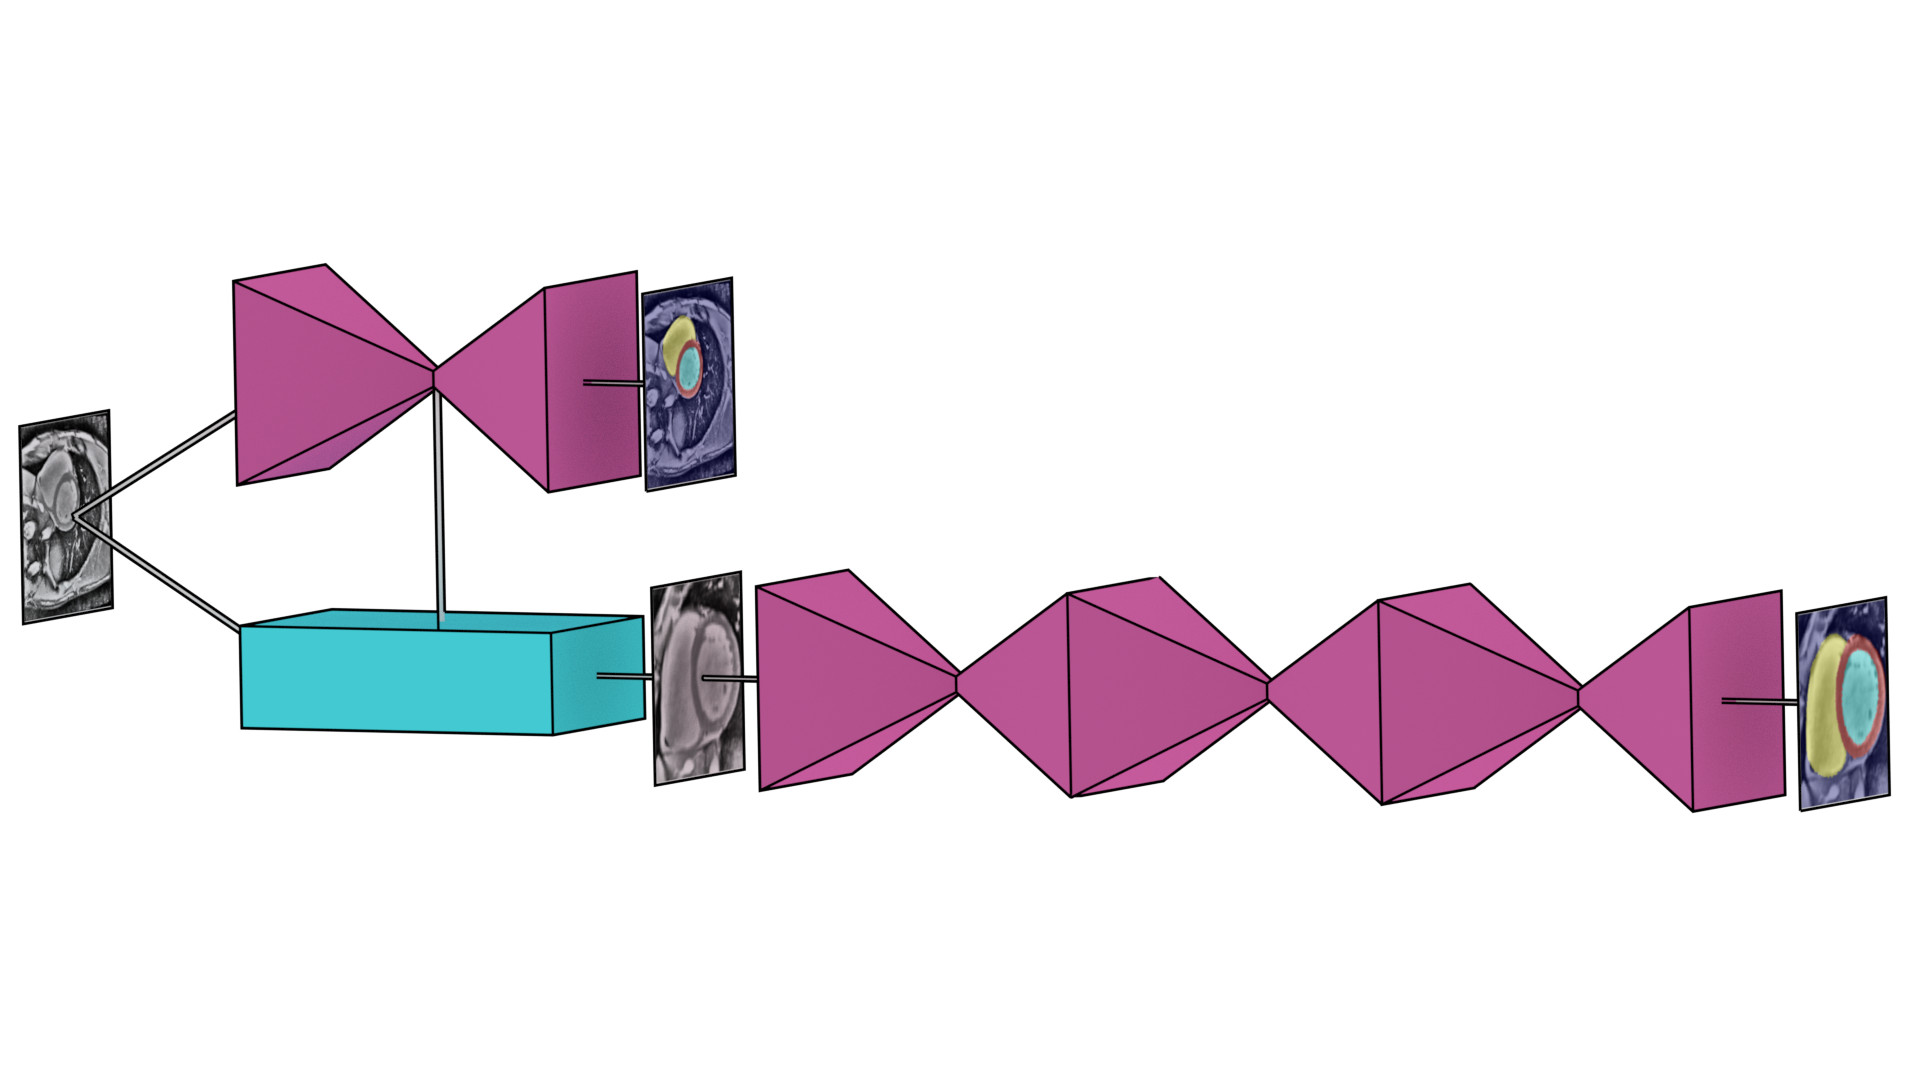
\includegraphics[clip, trim=0 260 0 260, width=1.0\textwidth]{./data/ohm-net-architecture.png}};

\node [anchor=south west] (a) at (0.025\tw,0.22\tw) {\large $\image$};
\node [anchor=south west] (b) at (0.35\tw,0.13\tw) {\large $\image^\prime$};
\node [anchor=south west] (c) at (0.35\tw,0.29\tw) {\large $S$};
\node [anchor=south west] (d) at (0.95\tw,0.13\tw) {\large $S^\prime$};
\node [anchor=south west] (e) at (0.17\tw,0.06\tw) {\large $\trans(\image, \tmat)$};

\draw [decorate,decoration={brace,amplitude=10pt},xshift=0pt,yshift=0pt](0.1275\tw,0.3\tw) -- (0.34\tw,0.3\tw) node [black,midway,xshift=0.0cm,yshift=+0.7cm] {(a) 粗分割模块};
\draw [decorate,decoration={brace,amplitude=10pt},xshift=0pt,yshift=0pt](0.3425\tw,0.045\tw) -- (0.1325\tw,0.045\tw) node [black,midway,xshift=0.0cm,yshift=-0.7cm] {(b) 变换模块};
\draw [decorate,decoration={brace,amplitude=10pt},xshift=0pt,yshift=0pt](0.4\tw,0.15\tw) -- (0.935\tw,0.15\tw) node [black,midway,xshift=0.0cm,yshift=+0.7cm] {(c) 细分割模块};
\end{tikzpicture}

\caption[\captiontitle]{\captiontitle{}.  (a) 将原始的 \SSFP{} 图像送入 \UNet{} 模块,得到一个粗分割输出 $S$.(b) 从该层 \UNet{} 中间(下采样)层输出的特征被用来给变换模块预测一个刚体仿射变换的参数 $\tmat$,该变换这可将输入图像变换到一个典型方向 $\image^\prime = \trans(\image, \tmat)$.(c) 这个变换后的图像就送入一个对堆叠的沙漏形网络对变换到典型方向的 $S^\prime$ 进行最后的细分割.需要说明的是,这里的所有模块都是从头开始端到端的训练的.}
\label{fig:omega-net-architecture}
\end{center}
\end{figure*}
